\documentclass[conference]{IEEEtran}

\usepackage[utf8]{inputenc}
\usepackage[T1]{fontenc}
\usepackage{cite}
\usepackage{amsmath}
\usepackage{booktabs}
\usepackage{array}
\usepackage{multirow}
\usepackage{tikz}
\usepackage{pgfplots}
\usepackage{url}
\usepackage{balance}
\usepackage{microtype}
\usetikzlibrary{arrows.meta,positioning,shapes.geometric,fit,backgrounds}
\usepgfplotslibrary{groupplots}
\pgfplotsset{compat=1.18}

\title{Design and Evaluation of a TCP Load Balancer\\with Threaded and Event-Driven I/O}

\author{
\IEEEauthorblockN{Sanskar Sharma, Prayag Kirar, and Piyush Satiya}
\IEEEauthorblockA{Department of Computer Science and Engineering\\
Indian Institute of Information Technology Vadodara\\
Gandhinagar, India\\
202451148, 202451134, 202451130}
\and
\IEEEauthorblockN{Prof. Rishabh Gupta}
\IEEEauthorblockA{Indian Institute of Information Technology Vadodara\\
Gandhinagar, India}
}

\begin{document}
\maketitle

\begin{abstract}
This paper presents the design, implementation, and measurement of a Layer-4 TCP load balancer written from scratch in C++17. The proxy routes each accepted TCP connection using round robin, least connections, or consistent hashing, and relays the resulting byte stream to one of three backends. Two connection-processing models are implemented: a blocking thread-per-connection proxy and a nonblocking Linux \texttt{epoll} event loop with optional \texttt{SO\_REUSEPORT} workers. The system includes active TCP reachability checks and bounded retries when an initial upstream connection fails. Evaluation covers active request throughput and latency, idle-connection capacity and process memory, routing properties, backend outage behavior, and TCP half-close correctness. In a short single-sample throughput sweep at 800 concurrent connections, four-worker epoll reached 253.1 k requests/s, compared with 165.9 k requests/s for the four-core threaded proxy. In the idle test, epoll established and held 30,000 connections with three process threads and 7.69 MB PSS. The threaded proxy passed at 5,000 connections but failed its active probe after establishing 9,213 of 10,000. These results demonstrate the resource-scaling difference in this test environment; the short unoptimized throughput measurements are preliminary and do not establish general production capacity.
\end{abstract}

\begin{IEEEkeywords}
TCP load balancing, epoll, thread-per-connection, event-driven I/O, failover, benchmarking
\end{IEEEkeywords}

\section{Introduction}
A TCP load balancer accepts a client connection, selects an upstream server, establishes a second connection, and forwards bytes in both directions. Even for this simple data path, connection-processing architecture can change the amount of per-connection memory, the number of scheduled threads, and the cost of handling many mostly idle sockets. Prior studies of server architectures motivate measuring these effects under stated workloads rather than assuming one concurrency model is universally superior \cite{pariag}. Load-balancing evaluations also show that routing behavior depends on request and backend characteristics \cite{rawls}.

This project implements a small Layer-4 proxy to study these concerns directly. It is intentionally a learning and measurement system, not a replacement for NGINX or HAProxy. It does not parse HTTP in the proxy path; HTTP is used by the included backend and benchmark clients.

The project makes four contributions:
\begin{itemize}
  \item A shared routing and backend-health layer with three connection-selection algorithms.
  \item Two proxy data planes: blocking relays using threads and a nonblocking \texttt{epoll} event loop.
  \item Initial-connect retry behavior and tests for routing, failover, and TCP half-close.
  \item A reproducible local benchmark suite that reports throughput, latency, idle capacity, process resources, and test outcomes.
\end{itemize}

\section{System Design}
\subsection{Architecture}
Fig.~\ref{fig:architecture} shows the main data path and the shared control components. The selected proxy core accepts a client TCP connection, asks the selected policy for one backend, connects upstream, and relays the stream. The health checker updates shared backend status. A failed initial upstream connection may cause a retry against another available backend; failures after stream relay begins are not replayed.

\begin{figure*}[t]
\centering
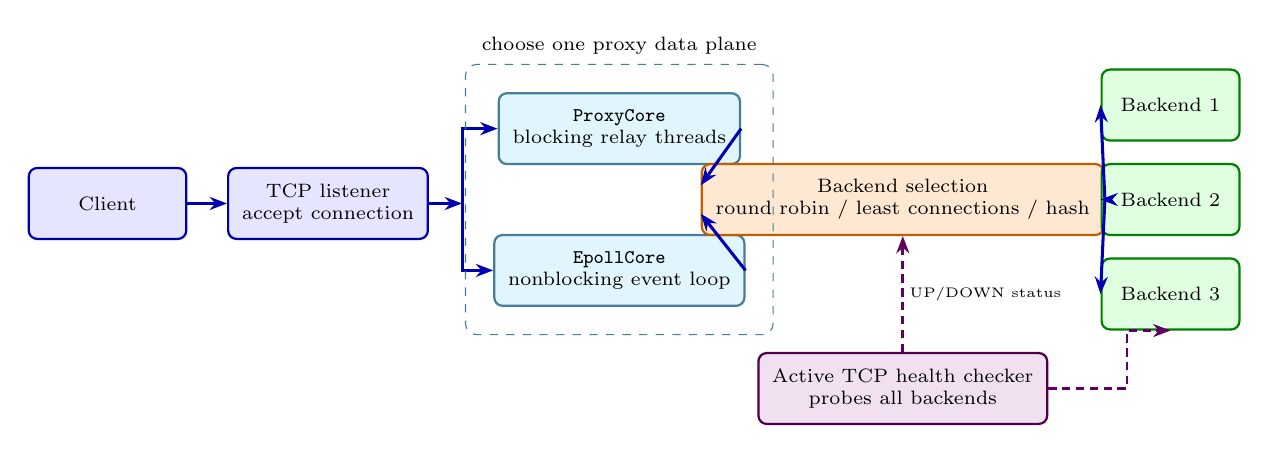
\begin{tikzpicture}[
  font=\scriptsize,
  nodebox/.style={draw,rounded corners=3pt,thick,align=center,minimum height=0.9cm,inner sep=5pt},
  io/.style={nodebox,fill=blue!10,draw=blue!65!black,minimum width=2.0cm},
  core/.style={nodebox,fill=cyan!12,draw=cyan!55!black,minimum width=2.75cm},
  policy/.style={nodebox,fill=orange!18,draw=orange!75!black,minimum width=2.65cm},
  backend/.style={nodebox,fill=green!12,draw=green!50!black,minimum width=1.75cm},
  control/.style={nodebox,fill=violet!12,draw=violet!60!black,minimum width=3.0cm},
  flow/.style={-{Stealth[length=2.2mm]},line width=1.1pt,draw=blue!70!black},
  ctlflow/.style={-{Stealth[length=2.2mm]},densely dashed,line width=1pt,draw=violet!75!black}
]
  \node[io] (client) at (0,0) {Client};
  \node[io] (listener) at (2.8,0) {TCP listener\\accept connection};
  \node[core] (threaded) at (6.5,0.95) {\texttt{ProxyCore}\\blocking relay threads};
  \node[core] (epoll) at (6.5,-0.85) {\texttt{EpollCore}\\nonblocking event loop};
  \node[policy] (router) at (10.1,0.05) {Backend selection\\round robin / least connections / hash};
  \node[backend] (b1) at (13.5,1.25) {Backend 1};
  \node[backend] (b2) at (13.5,0.05) {Backend 2};
  \node[backend] (b3) at (13.5,-1.15) {Backend 3};
  \node[control] (health) at (10.1,-2.35) {Active TCP health checker\\probes all backends};

  % Keep labels inside the boxes; unlabeled arrows make the data path unambiguous.
  \draw[flow] (client.east) -- (listener.west);
  \draw[flow] (listener.east) -- ++(0.42,0) coordinate (fork);
  \draw[flow] (fork) |- (threaded.west);
  \draw[flow] (fork) |- (epoll.west);
  \draw[flow] (threaded.east) -- ([yshift=0.18cm]router.west);
  \draw[flow] (epoll.east) -- ([yshift=-0.18cm]router.west);
  \draw[flow] (router.east) -- (b1.west);
  \draw[flow] (router.east) -- (b2.west);
  \draw[flow] (router.east) -- (b3.west);
  \draw[ctlflow] (health.north) -- node[right,font=\tiny,inner sep=2pt]{UP/DOWN status} (router.south);
  \draw[ctlflow] (health.east) -- ++(1.0,0) |- (b3.south);
  \node[draw=cyan!55!black,dashed,rounded corners=4pt,fit=(threaded)(epoll),inner sep=10pt,
        label={[font=\scriptsize]above:choose one proxy data plane}] {};
\end{tikzpicture}
\caption{Project architecture. The proxy forwards TCP bytes; HTTP appears only in the test responder and workload generator.}
\label{fig:architecture}
\end{figure*}

\subsection{Shared backend state and routing}
Each backend stores its configured endpoint, an atomic UP/DOWN state, active-connection and selection counters, and a cached IPv4 socket address. Successful address resolution is protected so multiple workers cannot race while initializing the same endpoint.

Round robin advances an atomic index and skips backends marked down. Least connections scans the active-connection counts under a mutex and selects the smallest observed value; connection setup and teardown update those atomic counts outside the selection lock, so the scan is a best-effort snapshot. Consistent hashing maps the client IPv4 string onto an ordered hash ring containing 100 virtual nodes per backend. The ring is constructed at startup. These algorithms choose a backend per TCP connection, not per HTTP request.

\subsection{Blocking thread-per-connection proxy}
\texttt{ProxyCore} accepts clients in a blocking loop and delegates connection setup to a handler thread. Once the upstream connection succeeds, two blocking relay directions run concurrently. Each relay uses an 8 KiB stack buffer, handles partial writes, and propagates TCP half-close. A shared connection tracker owns the client and backend descriptors and decrements the selected backend's active count after both relay directions finish.

\subsection{Epoll proxy}
\texttt{EpollCore} uses nonblocking client and backend sockets with level-triggered \texttt{epoll}. Each session maps both descriptors to shared session state. Two optional fixed-capacity 16 KiB buffers hold data that cannot yet be written to the destination. A buffer is allocated only when data needs buffering and released when drained. Reads are paused when the destination buffer is full, applying backpressure; write readiness is requested only while a connect is pending or buffered data remains. The \texttt{MAX\_EVENTS} array controls the number of ready descriptors returned per wait, not the number of connections the event loop can register \cite{epollman}.

With multiple workers, each loop owns an epoll descriptor and a listener bound to the same port using \texttt{SO\_REUSEPORT}. The operating system distributes new connections among these listeners. This is a set of independent event loops, not a shared loop or a general-purpose thread pool.

\subsection{Health checks and failover}
The health checker periodically performs a TCP connect to each backend and updates its UP/DOWN state. This proves listener reachability, not application-level health. Passive retry is a separate mechanism: if an initial upstream connect fails, the proxy may mark that backend down and try another backend, bounded to at most one attempt per configured backend. The connect timeout is 250 ms. The proxy does not retry an established stream because it cannot know whether bytes already delivered to the backend caused side effects.

\section{Experimental Method}
\subsection{Environment and workload}
The final recorded run used a 12-logical-CPU Linux host with 15 GiB RAM. The proxy was pinned to CPU 0 for single-core modes or CPUs 0--3 for four-worker modes; the load generator used CPUs 4--7 and the dummy backends CPUs 8--11. The host build used C++17 with warning flags and debug symbols but no compiler optimization flag. These are measurements of this host and build, not a production deployment claim.

The active HTTP workload used \texttt{wrk} 4.2.0 with four worker threads. Each configuration had one 1 s warmup and one 3 s measurement at 50, 200, or 800 concurrent keep-alive connections. The five modes were direct-backend control, single-worker epoll, four-worker epoll, one-core thread-per-connection, and four-core thread-per-connection. NGINX was omitted because the Docker service could not be run. RPS, latency percentiles, request/error counts, host CPU-set utilization, and sampled proxy-thread context switches were recorded. The CPU metric is utilization of the selected host CPU set, not proxy-only CPU utilization.

\subsection{Idle connections and memory}
The idle client opened connections in batches of 500, sent a keep-alive request, and read the complete HTTP response before counting each connection as established. It then sent 20 requests over a separate connection to measure active-request median latency while the idle connections were held for 5 s. The sampler ran during this hold and retained the snapshot with the largest descriptor count.

The process metrics are RSS, PSS, virtual address size (VmSize), thread count, and file descriptors. VmSize includes virtual reservations such as thread stacks; it is not resident RAM. RSS/PSS do not include kernel memory used by TCP sockets. Because these final idle runs were host-mode runs, cgroup memory and PID measurements are unavailable.

\subsection{Functional suites}
Routing properties were tested in five trials per algorithm. Round robin was checked against a 10/10/10 split over 30 new connections. Least connections was tested with held sessions that preloaded one backend before opening additional sessions. Consistent hashing was checked for stable backend selection for 30 client IPs across reconnects. These are property checks, not broad distribution studies.

Failover used 20 probes per second for 7 s per trial, with backend 9002 unavailable for 2.5 s; there were 20 trials with passive retry and 20 with passive retry disabled. A separate half-close test sent a 1 MiB request, closed only the client write side, and checked that the full response arrived with a matching SHA-256 digest in both proxy models.

\section{Results}
\subsection{Active throughput and latency}
Fig.~\ref{fig:throughput} shows how throughput changes with offered concurrency for every measured mode. Four-worker epoll led at each tested level. At 800 connections it measured 253.1 k requests/s, compared with 165.9 k requests/s for four-core threaded mode (Table~\ref{tab:throughput}). These are single short samples; the run does not estimate within-setting variability.

\begin{figure}[!t]
\centering
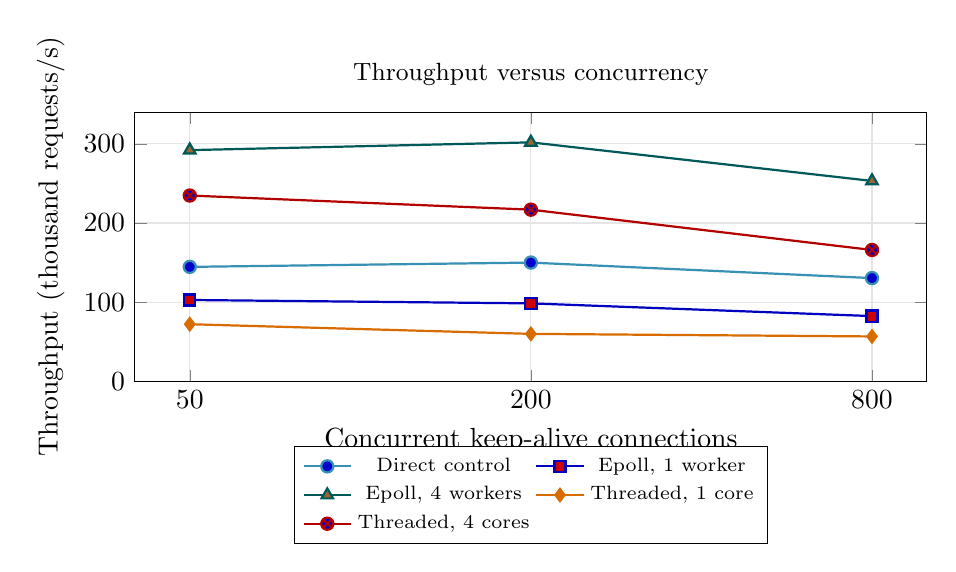
\begin{tikzpicture}
\begin{axis}[
  width=0.96\columnwidth, height=5.0cm,
  xmode=log, log basis x=10, xmin=40, xmax=1000,
  xtick={50,200,800}, xticklabels={50,200,800},
  xlabel={Concurrent keep-alive connections},
  ylabel={Throughput (thousand requests/s)},
  ymin=0, ymax=340, ymajorgrids=true, xmajorgrids=true,
  grid style={gray!20},
  legend style={at={(0.5,-0.24)},anchor=north,legend columns=2,font=\scriptsize},
  title={Throughput versus concurrency}, title style={font=\small}
]
\addplot+[thick,cyan!70!black,mark=*,mark size=2.2pt] coordinates {(50,144.596) (200,150.009) (800,130.427)};
\addlegendentry{Direct control}
\addplot+[thick,blue!75!black,mark=square*,mark size=2.0pt] coordinates {(50,102.771) (200,98.499) (800,82.423)};
\addlegendentry{Epoll, 1 worker}
\addplot+[thick,teal!70!black,mark=triangle*,mark size=2.4pt] coordinates {(50,292.052) (200,301.864) (800,253.129)};
\addlegendentry{Epoll, 4 workers}
\addplot+[thick,orange!85!black,mark=diamond*,mark size=2.2pt] coordinates {(50,72.157) (200,59.958) (800,56.715)};
\addlegendentry{Threaded, 1 core}
\addplot+[thick,red!70!black,mark=otimes*,mark size=2.2pt] coordinates {(50,234.714) (200,216.858) (800,165.938)};
\addlegendentry{Threaded, 4 cores}
\end{axis}
\end{tikzpicture}
\caption{All 15 active-throughput observations. Lines connect the three offered concurrency levels; each point is one 3 s measurement.}
\label{fig:throughput}
\end{figure}

\begin{table}[!t]
\caption{800-Connection Results}
\label{tab:throughput}
\centering
\footnotesize
\begin{tabular}{lrr}
\toprule
Mode & RPS (k) & P99 (ms) \\
\midrule
Direct control & 130.4 & 8.17 \\
Epoll, 1 worker & 82.4 & 13.28 \\
Epoll, 4 workers & 253.1 & 8.81 \\
Threaded, 1 core & 56.7 & 29.39 \\
Threaded, 4 cores & 165.9 & 22.03 \\
\bottomrule
\end{tabular}
\end{table}

At 800 connections, four-worker epoll had a lower P99 than four-core threaded mode in this run. The single-worker epoll run did not outperform the direct control in RPS and reached a higher CPU-set busy percentage. This is a result for this build, host, and workload, not a general guarantee about epoll.

\subsection{Idle connection capacity and process memory}
Fig.~\ref{fig:idle_resources} plots resource growth against the number of established connections instead of comparing unrelated categories. Epoll passed all three targets. The threaded proxy passed 5,000 but did not complete its 10,000 target: it established 9,213 and failed the active probe. Its 150.9 GiB VmSize is virtual address space, not physical memory.

\begin{figure*}[!t]
\centering
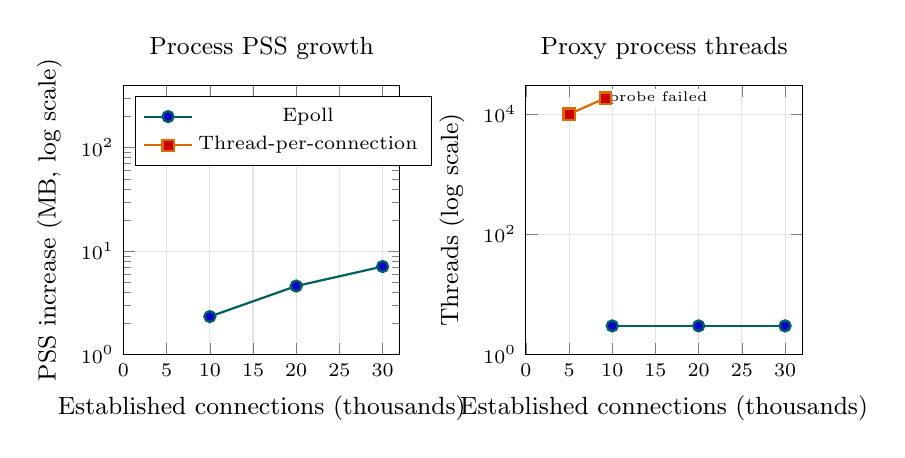
\begin{tikzpicture}
\begin{groupplot}[
  group style={group size=2 by 1,horizontal sep=1.6cm},
  width=0.42\textwidth,height=5.0cm,
  xmin=0,xmax=32,xtick={0,5,10,15,20,25,30},
  xlabel={Established connections (thousands)},
  xmajorgrids=true,ymajorgrids=true,grid style={gray!20},
  tick label style={font=\scriptsize},
  label style={font=\small},
  title style={font=\small}
]
\nextgroupplot[
  title={Process PSS growth},ylabel={PSS increase (MB, log scale)},
  ymode=log,ymin=1,ymax=400,
  legend style={at={(0.04,0.96)},anchor=north west,font=\scriptsize}
]
\addplot+[thick,teal!75!black,mark=*] coordinates {(10,2.33) (20,4.60) (30,7.10)};
\addlegendentry{Epoll}
\addplot+[thick,orange!85!black,mark=square*] coordinates {(5,121.03) (9.213,226.82)};
\addlegendentry{Thread-per-connection}
\nextgroupplot[
  title={Proxy process threads},ylabel={Threads (log scale)},
  ymode=log,ymin=1,ymax=30000
]
\addplot+[thick,teal!75!black,mark=*] coordinates {(10,3) (20,3) (30,3)};
\addplot+[thick,orange!85!black,mark=square*] coordinates {(5,10003) (9.213,18429)};
\node[font=\tiny,anchor=west,fill=white,inner sep=1pt] at (axis cs:9.213,18429) {probe failed};
\end{groupplot}
\end{tikzpicture}
\caption{Process-resource scaling during the 5 s idle hold. The threaded 10k target stopped at 9,213 established connections and failed its active probe.}
\label{fig:idle_resources}
\end{figure*}

\begin{table}[!t]
\caption{Idle-Test Resource Snapshot}
\label{tab:idle}
\centering
\footnotesize
\begin{tabular}{lrrl}
\toprule
Mode / established & Threads & PSS growth (MB) & Outcome \\
\midrule
Epoll / 10,000 & 3 & 2.33 & Pass \\
Epoll / 20,000 & 3 & 4.60 & Pass \\
Epoll / 30,000 & 3 & 7.10 & Pass \\
Threaded / 5,000 & 10,003 & 121.03 & Pass \\
Threaded / 9,213* & 18,429 & 226.82 & Probe failed \\
\bottomrule
\end{tabular}
\end{table}

At 30,000 connections, epoll used 3 process threads and 60,005 descriptors. At 5,000 connections, the threaded process used 10,003 threads. Its incomplete 10k-target run reached 18,429 threads. PSS does not include kernel TCP socket memory; VmSize includes virtual reservations such as thread stacks and is not resident RAM.

\subsection{Routing policy properties}
The routing suite checked behavior rather than ranking application performance. Round robin produced the expected 10/10/10 distribution over 30 connections in each of five runs. The least-connections scenario opened new sessions after deliberately preloading one backend. Consistent hashing selected the same backend for each of 30 client IPs across reconnects. These checks do not rank the algorithms under heterogeneous request costs or backend capacities.

\begin{table}[!t]
\caption{Functional Checks}
\label{tab:functional}
\centering
\footnotesize
\begin{tabular}{p{0.25\columnwidth}p{0.63\columnwidth}}
\toprule
Check & Observed result \\
\midrule
Round robin & 10/10/10 over 30 connections in all 5 runs \\
Least connections & New held sessions distributed around a preloaded backend; 5 runs \\
Consistent hashing & 30 client IPs retained backend affinity across reconnects; 5 runs \\
TCP half-close & Threaded and epoll relayed the complete 1 MiB request and 1,048,608-byte response; hashes matched \\
\bottomrule
\end{tabular}
\end{table}

\subsection{Failover under a backend outage}
Fig.~\ref{fig:failover} shows every trial's number of failed probes after the backend was killed. With passive retries disabled, the suite recorded a mean of 3.65 failed probes per trial (standard deviation 2.16; 20 trials). Passive retries recorded zero dropped probes in all 20 trials. This result applies to the tested outage schedule and probe rate.

\begin{figure}[!t]
\centering
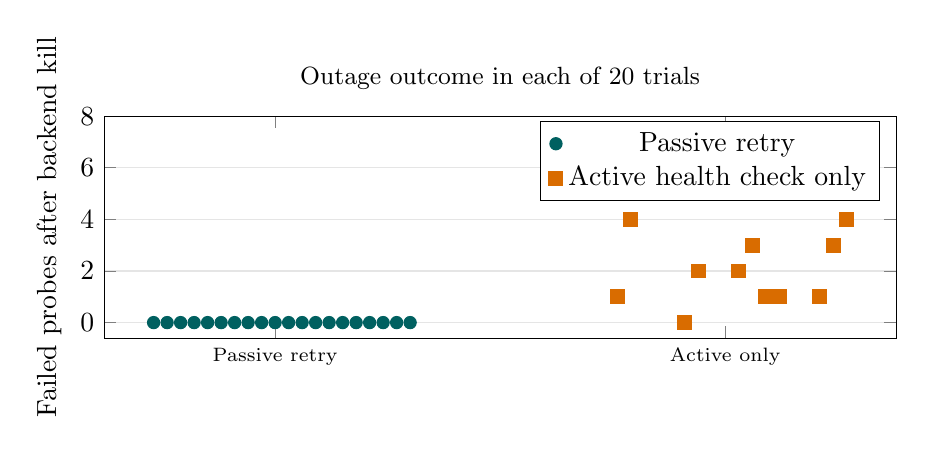
\begin{tikzpicture}
\begin{axis}[
  width=0.96\columnwidth,height=4.4cm,
  xmin=-0.38,xmax=1.38,ymin=-0.6,ymax=8,
  xtick={0,1},xticklabels={Passive retry,Active only},
  xticklabel style={font=\scriptsize},
  ylabel={Failed probes after backend kill},
  ytick={0,2,4,6,8},ymajorgrids=true,grid style={gray!20},
  title={Outage outcome in each of 20 trials},title style={font=\small}
]
\addplot[only marks,mark=*,mark size=2.2pt,teal!75!black] coordinates {
  (-0.27,0) (-0.24,0) (-0.21,0) (-0.18,0) (-0.15,0)
  (-0.12,0) (-0.09,0) (-0.06,0) (-0.03,0) (0,0)
  (0.03,0) (0.06,0) (0.09,0) (0.12,0) (0.15,0)
  (0.18,0) (0.21,0) (0.24,0) (0.27,0) (0.30,0)
};
\addlegendentry{Passive retry}
\addplot[only marks,mark=square*,mark size=2.5pt,orange!85!black] coordinates {
  (0.73,6) (0.76,1) (0.79,4) (0.82,6) (0.85,5)
  (0.88,5) (0.91,0) (0.94,2) (0.97,5) (1.00,6)
  (1.03,2) (1.06,3) (1.09,1) (1.12,1) (1.15,5)
  (1.18,7) (1.21,1) (1.24,3) (1.27,4) (1.30,6)
};
\addlegendentry{Active health check only}
\end{axis}
\end{tikzpicture}
\caption{Jitter separates overlapping trial markers at zero and preserves the individual trial outcomes.}
\label{fig:failover}
\end{figure}

\section{Discussion and Limitations}
The clearest measured distinction is resource scaling for mostly idle connections. Epoll kept 30,000 client and upstream connections using three process threads, while the threaded design required roughly two relay threads per proxied session and could not pass its 10,000-target probe. This is consistent with the design difference: epoll keeps per-connection session state, while the threaded model also pays for many kernel threads and their stacks.

The throughput data is less conclusive. Each point is one three-second sample, the build had no optimization flag, and CPU utilization measures selected host CPU sets rather than proxy-only CPU. The local dummy backend returns a small fixed response and is not representative of application workloads. NGINX could not be included in the final run. The algorithm checks are functional rather than statistical comparisons. Process RSS/PSS omit kernel socket memory, and the threaded 10k row is a failed partial run rather than a successful capacity point.

Accordingly, this paper reports results from this implementation, host, build, and workload. It does not claim that this project outperforms production load balancers or that the measurements predict deployment capacity. Useful next experiments would use optimized builds, repeated randomized trials, a wider payload and backend-service-time matrix, and a direct NGINX or HAProxy comparison under identical resource limits.

\section{Conclusion}
We implemented a from-scratch TCP load balancer with three routing algorithms, active TCP health checks, bounded initial-connect retry, a blocking thread-per-connection proxy, and a Linux epoll proxy. The final short evaluation exercised throughput, tail latency, idle connection scaling, process resources, routing properties, failover, and TCP half-close. In the recorded environment, the multi-worker epoll model sustained 30,000 idle connections with low process memory and substantially fewer threads than the threaded model. Four-worker epoll also produced the highest measured throughput in the short active sweep. These are useful results for understanding the implementation tradeoffs, with the limitations above defining the boundary of the claims.

\balance
\begin{thebibliography}{3}
\bibitem{pariag}
D. Pariag, T. Brecht, A. Harji, P. A. Buhr, and A. Shukla, ``Comparing the Performance of Web Server Architectures,'' in \emph{Proc. EuroSys}, 2007, pp. 231--243, doi: 10.1145/1272998.1273021.

\bibitem{rawls}
C. Rawls and M. A. Salehi, ``Load Balancer Tuning: Comparative Analysis of HAProxy Load Balancing Methods,'' arXiv:2212.14198, 2022. [Online]. Available: \url{https://arxiv.org/abs/2212.14198}

\bibitem{epollman}
Linux man-pages project, ``epoll(7)---I/O event notification facility.'' [Online]. Available: \url{https://man7.org/linux/man-pages/man7/epoll.7.html}. Accessed: Oct. 26, 2026.
\end{thebibliography}

\end{document}
